\documentclass[aspectratio=169]{beamer}
\usepackage[utf8]{inputenc}
\usepackage{graphics}
\usepackage[english,serbian]{babel}
\usepackage{booktabs} %za tabelu

\usetheme[sectionstyle=style2]{trigon}
\titlegraphic{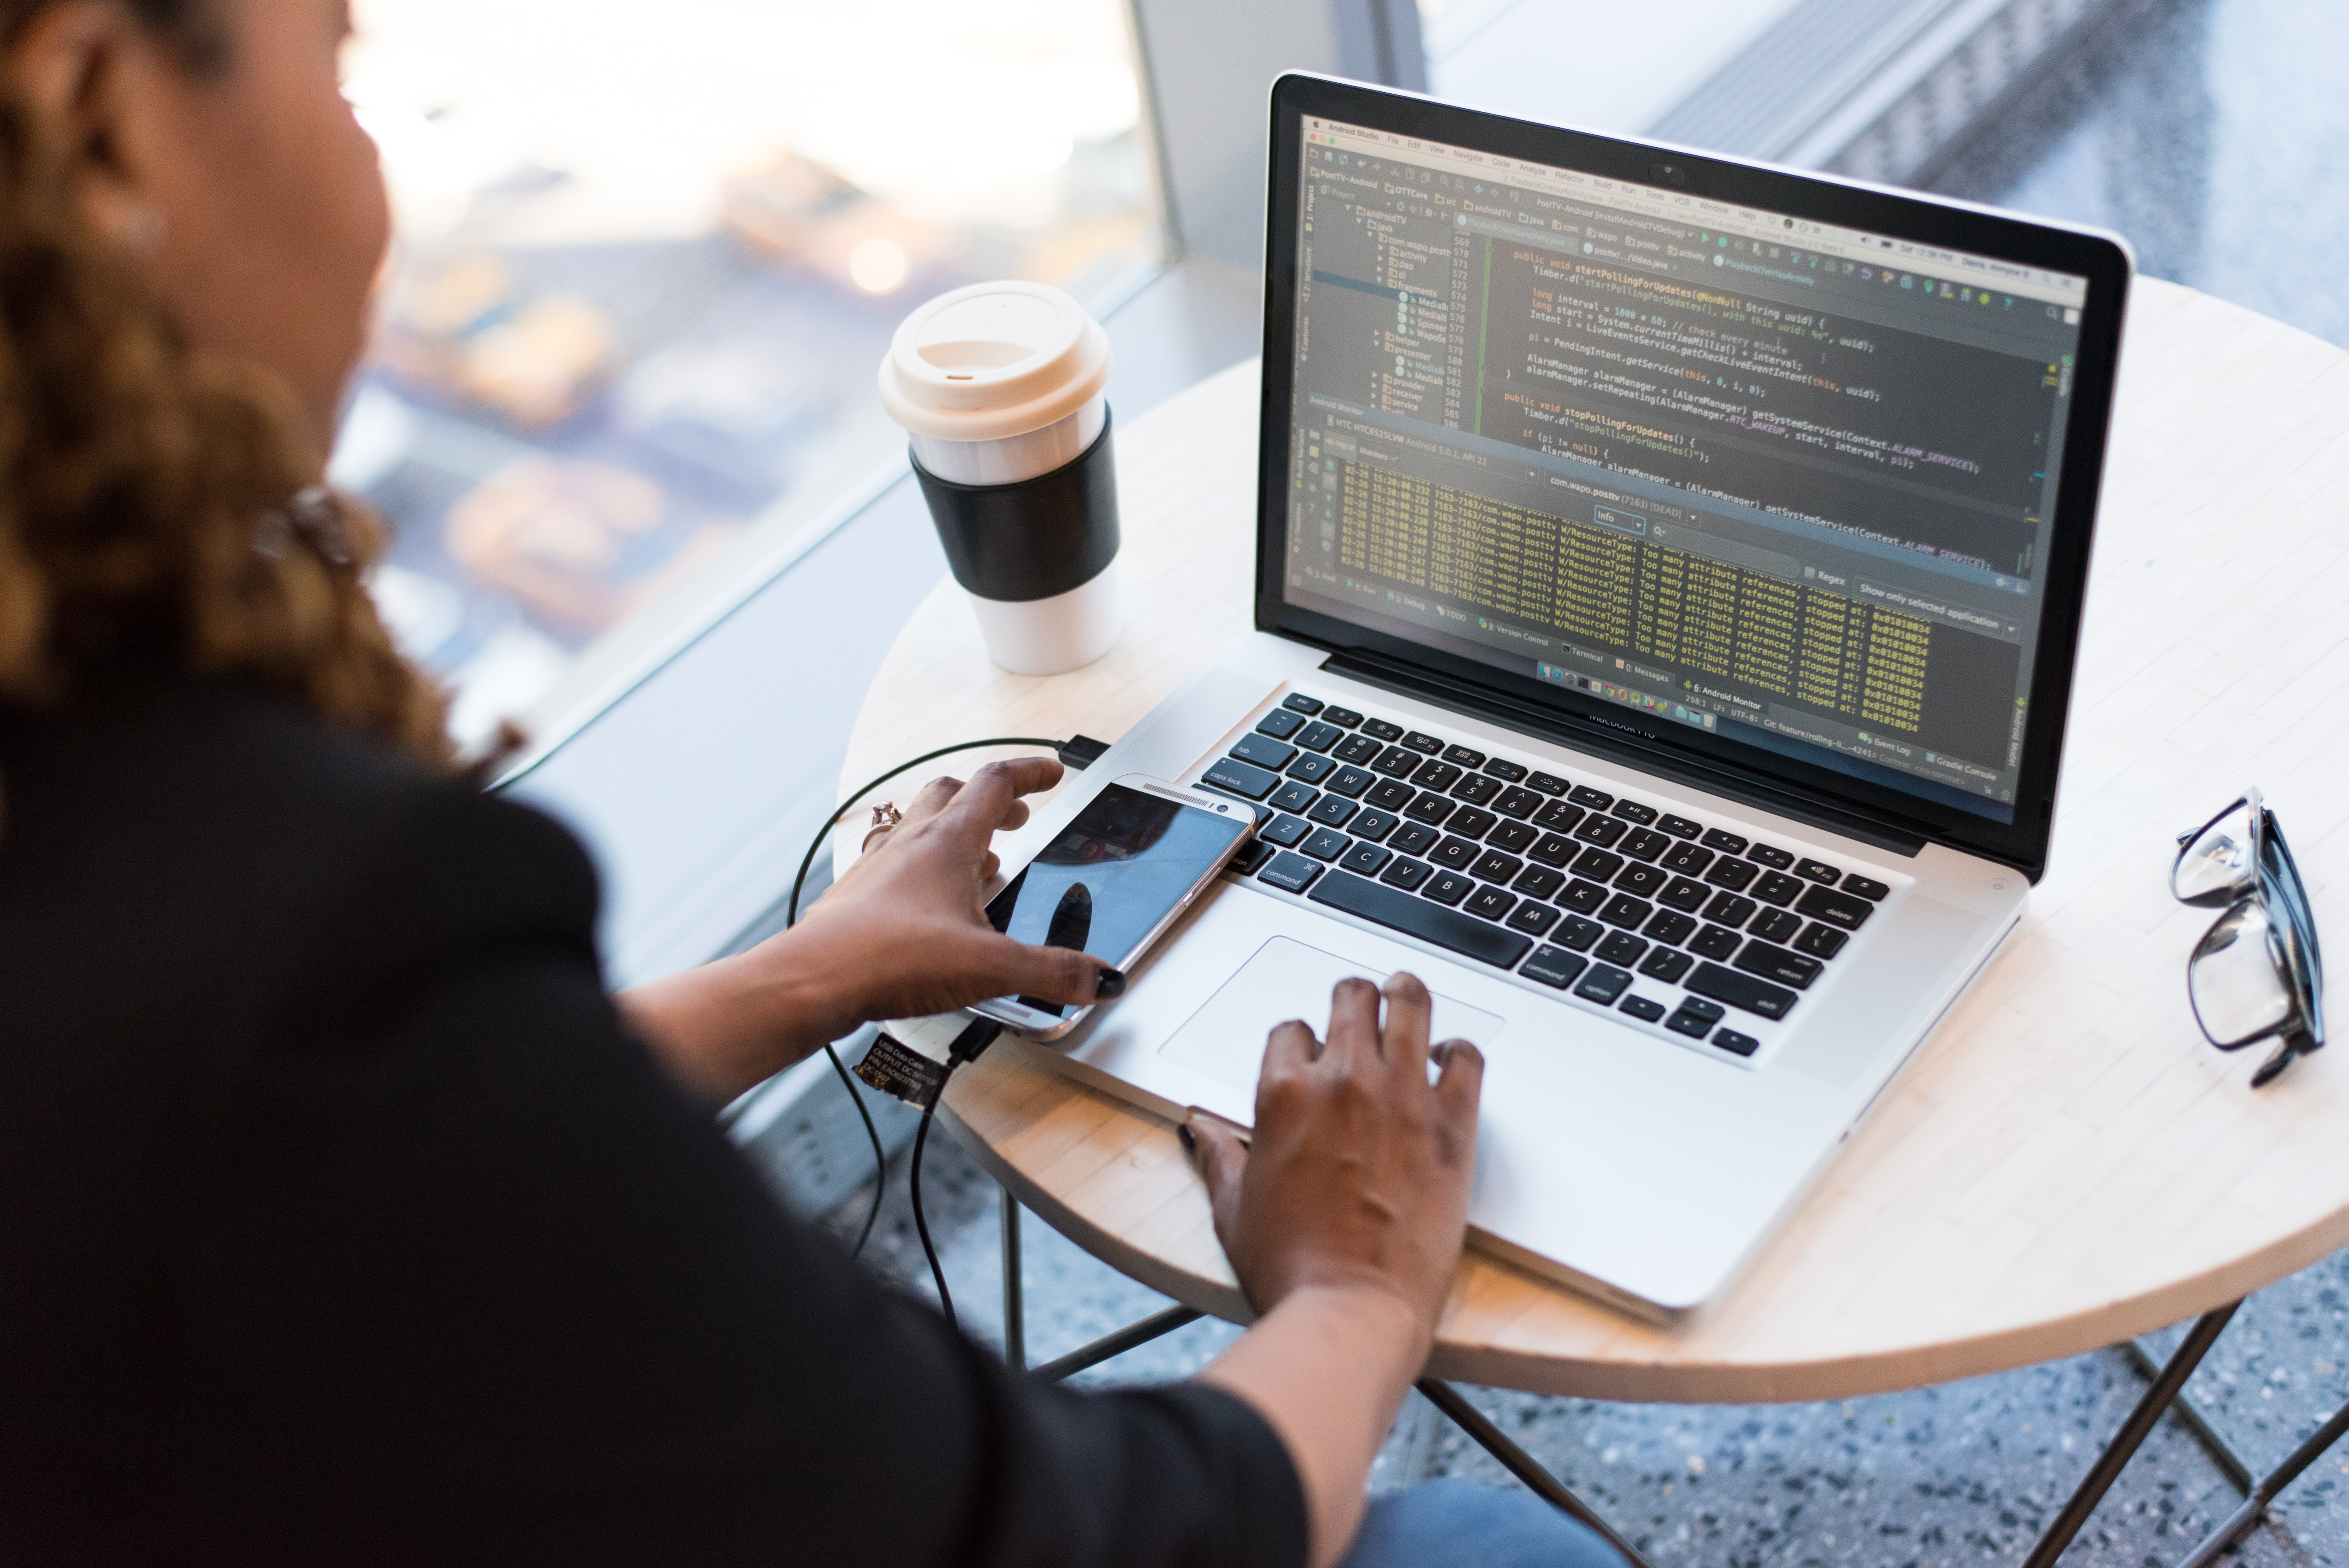
\includegraphics[height=\paperheight]{slika1.jpg}} %slika na prvom slajdu
\biglogo{LOGO-1.png} %logo na pocetnom slajdu

\title{Žene u računarstvu}
\author{ Zorana Jevtić \and Bojana Zagorac\\  \and Miloš Bigović  \and Jelena Veličković\\}
\date{Decembar 2022}



%==============================================================================
%                               BEGIN DOCUMENT
%==============================================================================


\begin{document}

\titleframe  %za pravljenje pocetnog slajda
\setbeamertemplate{frame footer}{Zorana Jevtić, Bojana Zagorac, Miloš Bigović, Jelena Veličković}

%==============================================

\begin{frame}{Sadržaj}
  \setbeamertemplate{section in toc}[sections numbered]
  \tableofcontents[hideallsubsections]
\end{frame}

%==============================================
\section{Ada Bajron}
%==============================================



%==============================================
\section{Margaret Hamilton}
%==============================================
\begin{frame}{Biografija}

    \begin{itemize}
        \item<1-> Margaret Hamilton je bila jedan od prvih programera kompjuterskog softvera.
        
        \item<2-> Studirala je matematiku i filozofiju na Earlham koledžu u Ričmondu.
        
        \item<3->Iako je Margaret planirala da studira apstraktnu matematiku na Univerzitetu Brandeis, prihvatila je posao na Tehnološkom institutu u Masačusetsu (MIT).
    \end{itemize}


\end{frame}
\begin{frame}{Karijera}

    \begin{itemize}
        \item<1-> Početkom 1960-ih Hamiltonova se pridružila MIT-ovoj Linkoln laboratoriji, gde je bila uključena u projekat Poluautomatsko zemaljsko okruženje, prvi američki sistem protivvazdušne odbrane.
        
        \item<2->Hamilton je zatim radila u kompaniji ''MIT’s Instrumentation Laboratory'', koja je obezbedila aeronautičku tehnologiju za NASA-u. Predvodila je tim koji je imao zadatak da razvije softver za sisteme navođenja i kontrole komandnih i lunarnih modula misija ''Apolo'' u letu.
        
        \item<3-> Sama Margaret se posebno koncentrisala na softver za otkrivanje sistemskih grešaka i za oporavak informacija u slučaju pada računara. Oba ta elementa bila su presudna tokom misije Apolo 11 (1969), koja je odvela astronaute Nila Armstronga i Baza Oldrina na Mesec.
    \end{itemize}


\end{frame}
\begin{frame}
  
    \begin{columns}
        \column{0.5\textwidth}
        \begin{figure}[h]
    \centering
    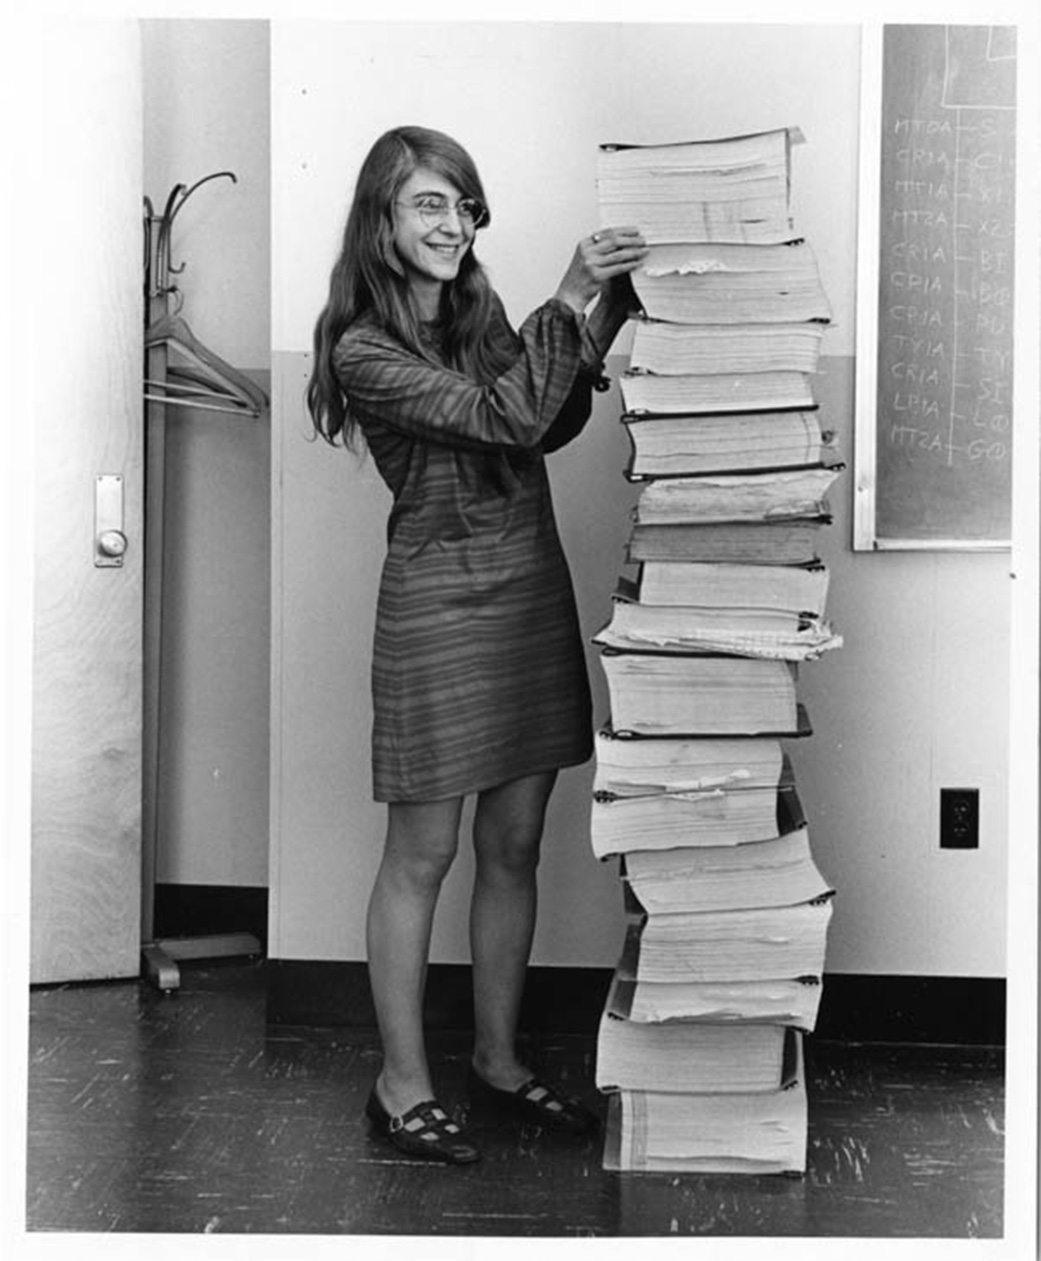
\includegraphics[width = .4\textwidth]{margaret_hamilton5.jpg}
    \caption{Margaret Hamilton}
    \label{fig:my_label}
\end{figure}

        \column{0.5\textwidth}
        \begin{block}{Dostignuća}
            \begin{itemize}
                \item<1->Bila je jedna od osnivača kompanije Higher Order Software 1976. godine.

                \item<2->Osnovala je Hamilton Technologies.

                \item<3-> Hamilton je bila dobitnica raznih počasti, uključujući NASA-inu nagradu o izuzetnom dostignuću.
                
            \end{itemize}
        \end{block}        
    \end{columns}
   
\end{frame}


%==============================================
\section{Eniac programeri}
%==============================================



%==============================================
\section{Zastupljenost žena u IT sektoru}
%==============================================

\begin{frame}{Statistika}

    \begin{itemize}
        \item<1-> Posle Drugog svetskog rata, programiranje je postalo popularnije među oba pola.
        
        \item<2->Do sredine ‘80-ih godina procenat žena na kompjuterskim naukama rastao je veoma brzo.
        
        \item<3-> Kada su žene počele u ovoj oblasti da čine više od \alert{37\%} studenata, procenat je počeo naglo da pada sve do danas. 
    \end{itemize}

    \begin{table}[h]
        \centering
        \begin{tabular}{c|c}
        \toprule
                Godina    & procenat žena u IT-u \\ 
        \midrule
                1984       & 37\%  \\ 
                1990-2010  & 18\%  \\ 
                2019       & 13\%  \\ 
        \bottomrule
        \end{tabular}
    \end{table}

\end{frame}

%------------------------------------------------

{\usebackgroundtemplate{
\includegraphics[width=\paperwidth, height=\paperheight]{slika8.jpg}}
\begin{frame}
  
    \begin{columns}
        \column{0.5\textwidth}
        \begin{block}{Zasto tako malo žena ulazi u IT}
            \begin{itemize}
            \item<1-> Žene su manje zainteresovane?
            \item<2-> Kultura, štetni stereotipi
            \item<3-> Nedostatak podrške na školskom nivou 
            \item<4-> Nedostatak ženskih uzora
            \end{itemize}
        \end{block}  

        \column{0.5\textwidth}
        \begin{block}{Budućnost žena u IT-u}
            \begin{itemize}
                \item<5-> Industrija kompjuterskih nauka raste izuzetnom brzinom

                \item<6-> Da bi se ovaj problem rešio potrebno je da se žene u IT-u više promovišu

                \item<7-> Twitter, Instagram, TikTok su uveli razne heštegove kojim podržavaju i podstiču rad žena u IT kompanijama 
            \end{itemize}
        \end{block}        
    \end{columns}
   
\end{frame}
}

%=================================================

{\usebackgroundtemplate{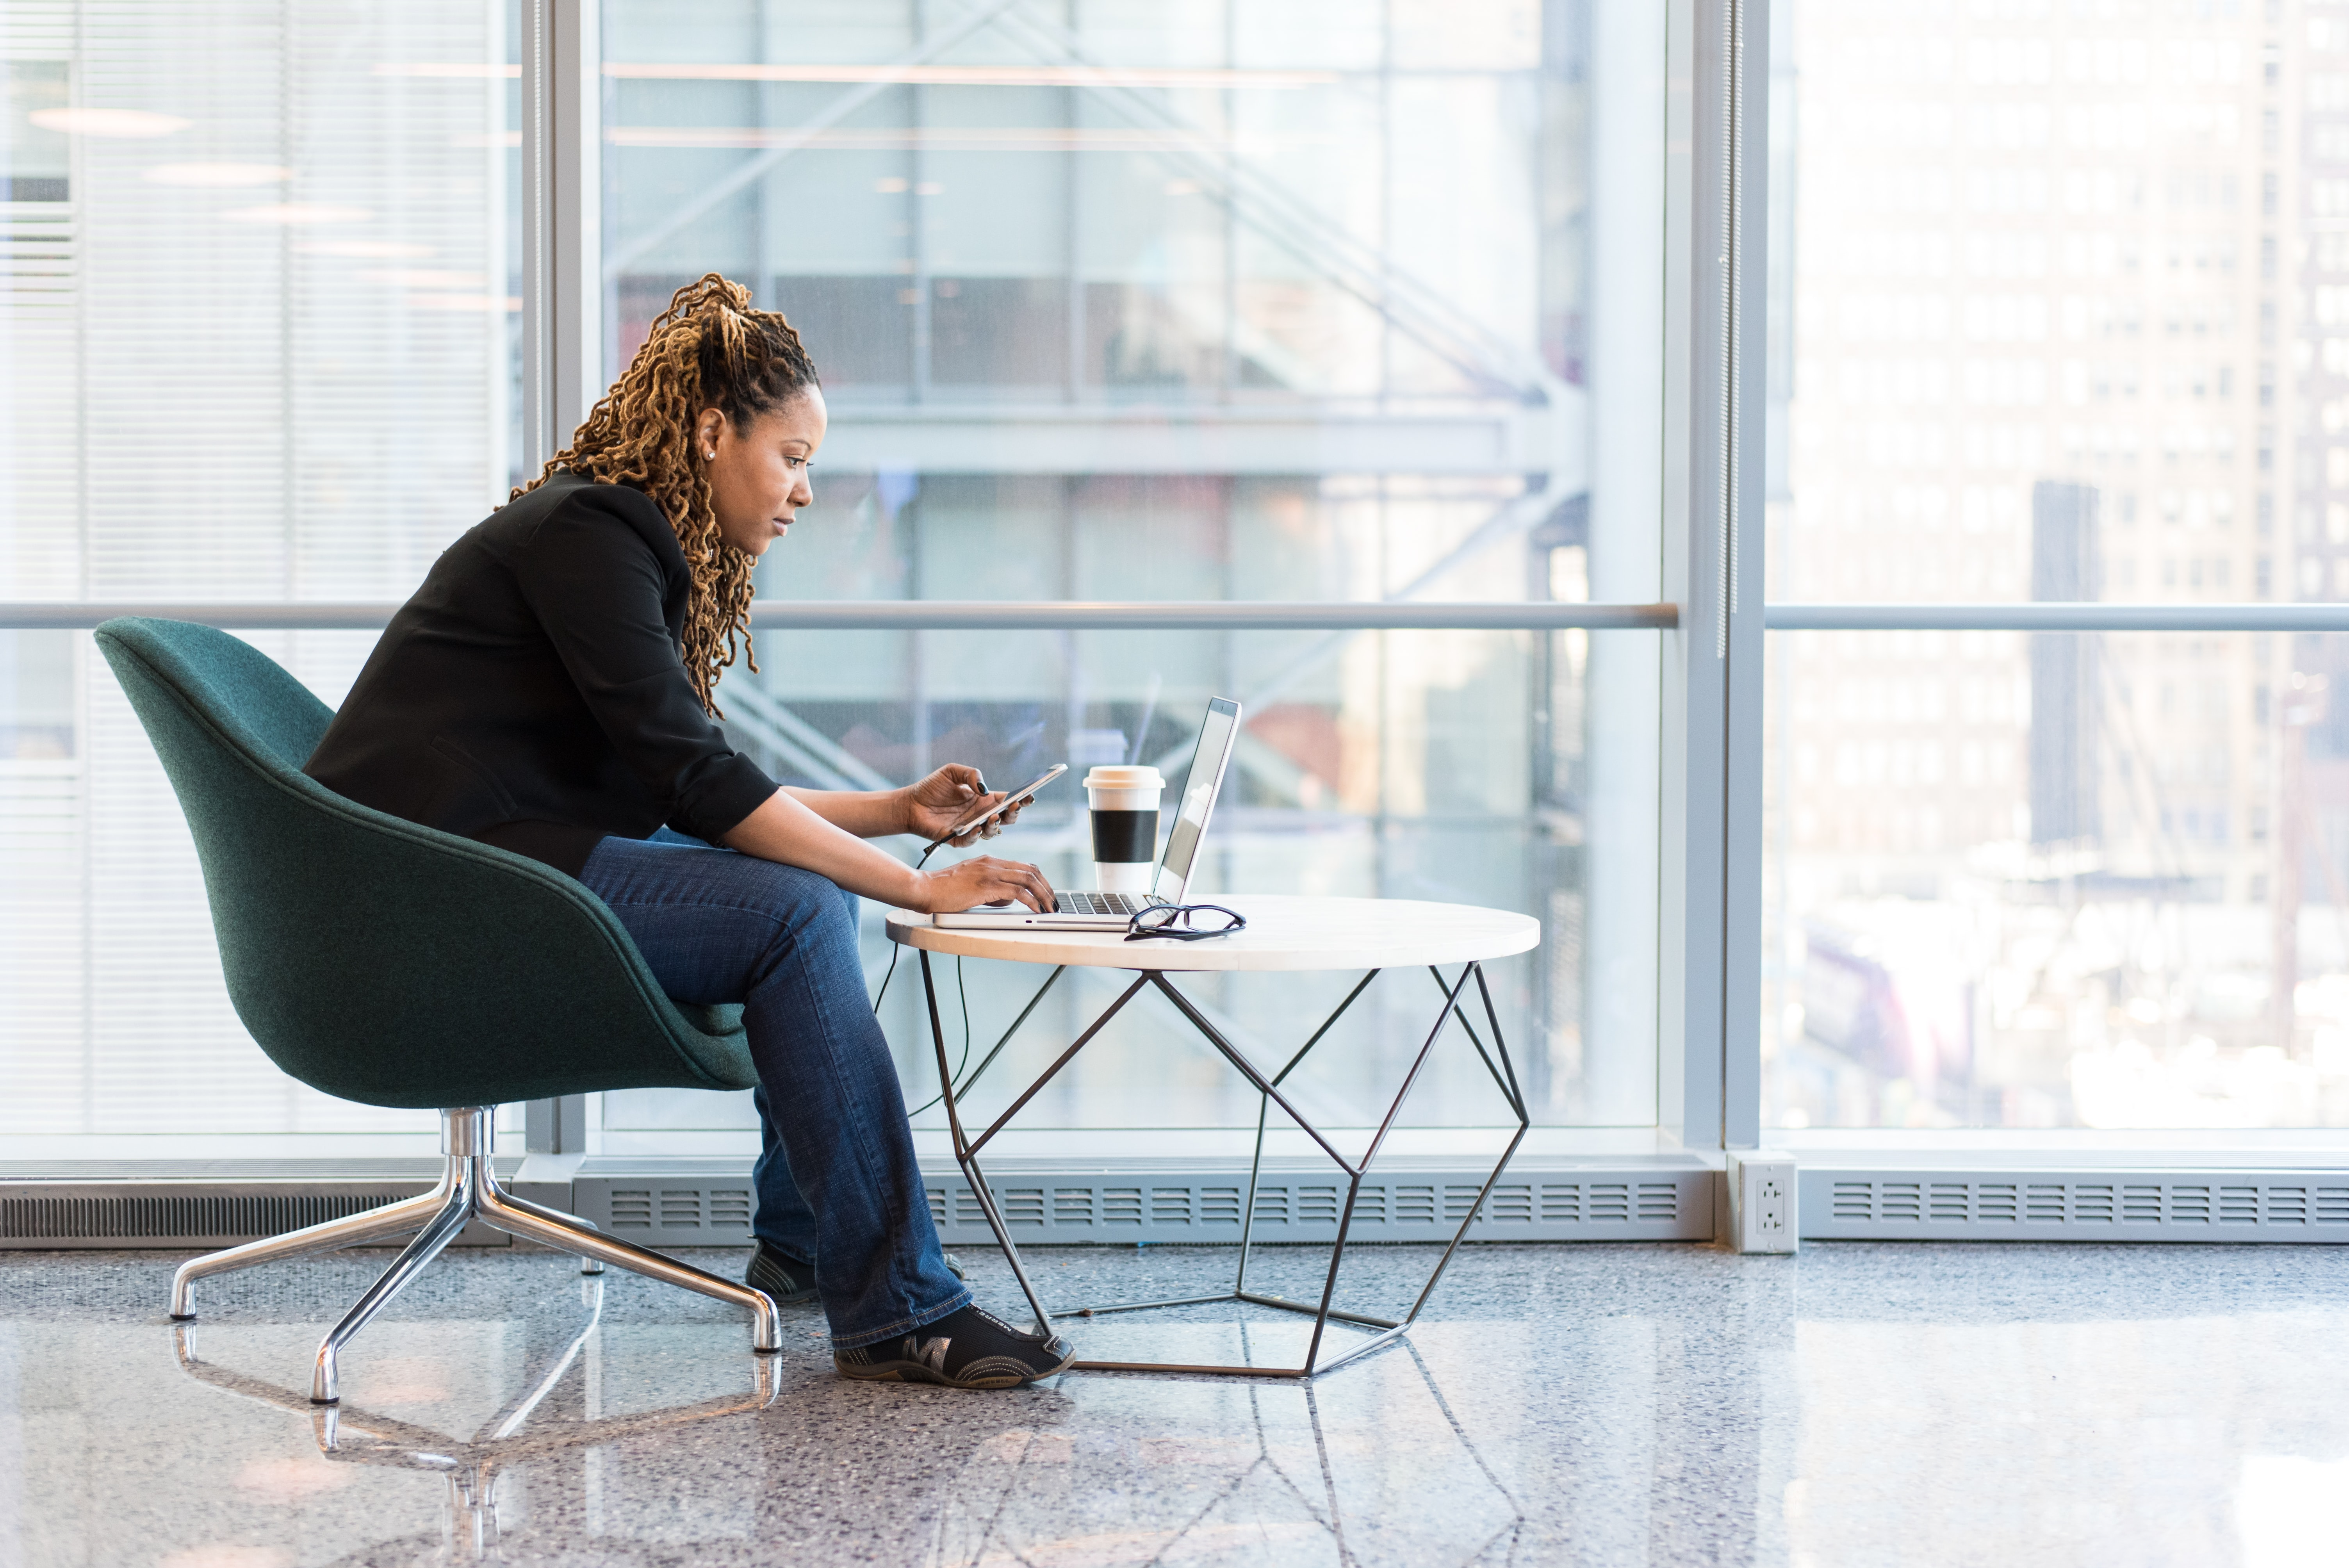
\includegraphics[width=\paperwidth, height=\paperheight]{slika2.jpg}}
\begin{frame}
    \centering
   \textbf{\Huge{KRAJ}} 
\end{frame}
}

\end{document}
